\documentclass[../main.tex]{subfiles}
\begin{document}
\newpage
\hypertarget{q14}{\section{Подграфик функции, площадь подграфика функции. Площадь криволинейной трапеции, ограниченной двумя графиками. Площадь эллипса.}}
Если \( f \geq 0\quad\), то \( \displaystyle\int\limits_{ a}^{ b}f(x)dx=S\left( \left[ a,b\right],f\right)\) - \emph{площадь подграфика} функции \( f\).

\begin{thm}[Площадь криволинейной трапеции]
    \( \Let \; f,g\in C\left[ a,b\right],\) \[ \forall \;x \in \left[ a,b\right]\; f\left( x\right) \leq g\left( x\right),\quad E = \left\{ \left( x,y\right): \; x \in \left[ a,b\right], \; f\left( x\right) \leq y \leq g\left( x\right)\right\}\]
    Тогда \[ S\left( E\right) = \displaystyle\int\limits_{ a}^{ b} f\left( x\right)-g\left( x\right)dx\]
\end{thm}
\begin{proof}
    
    ~

    \InsertBoxR{0}{
        \begin{minipage}[t]{6cm} 
            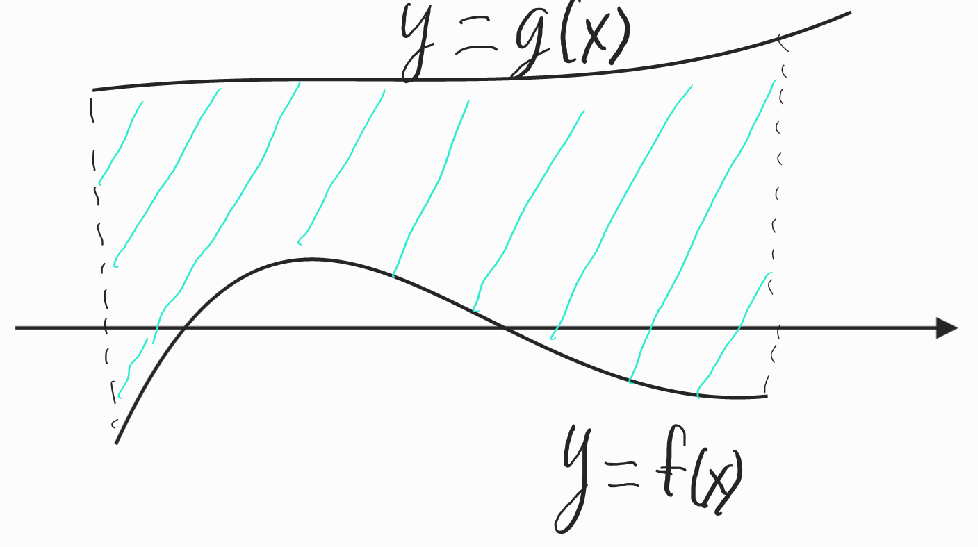
\includegraphics[width=\linewidth]{14_curved.pdf} 
        \end{minipage}
    }
    Этот факт очень простой, если \( f, g \geq 0\), потому что тогда площади их подграфиков - это интегралы, а про них мы всё знаем. Если же \(f\) или \( g < 0\), то мы можем просто передвинуть их так, чтобы на нужном отрезке они 
    обе были \( \geq 0\), а площадь сохранится, т.к. она сохраняется при движении. 
    
    \[ \Let \; m= \min\limits_{ \left[ a,b\right]} f\left( x\right),\quad f_1\left( x\right)=f\left( x\right)-m, \quad f_2\left( x\right)=f\left( x\right)-m\]
    \[ E_1=\left\{ \left( x,y\right):\; f_1\left( x\right) \leq y \leq g_1\left( x\right)\right\}=E+ \left( 0,m\right)\quad\text{-  сдвиг на вектор}\]
    \( S(E_1)=S(E)\), т.к. площадь инвариантна относительно изометрий, в том числе и относительно параллельного переноса. При этом \( f_1 \geq 0,\; g \geq 0\), поэтому
    \[ S\left( E\right)=S\left( \left[ a,b\right],g_1\right)-S\left( \left[ a,b\right],f_1\right)= \displaystyle\int\limits_{ a}^{ b} \left( g\left( x\right)-m\right)dx- \displaystyle\int\limits_{ a}^{ b} \left( f\left( x\right)-m\right)dx= \displaystyle\int\limits_{ a}^{ b} g\left( x\right)-f\left( x\right)dx\]
\end{proof}

\begin{example}[\hypertarget{elips_area}{Площадь эллипса}]

    ~

    \InsertBoxL{0}{
        \begin{minipage}[t]{6cm} 
            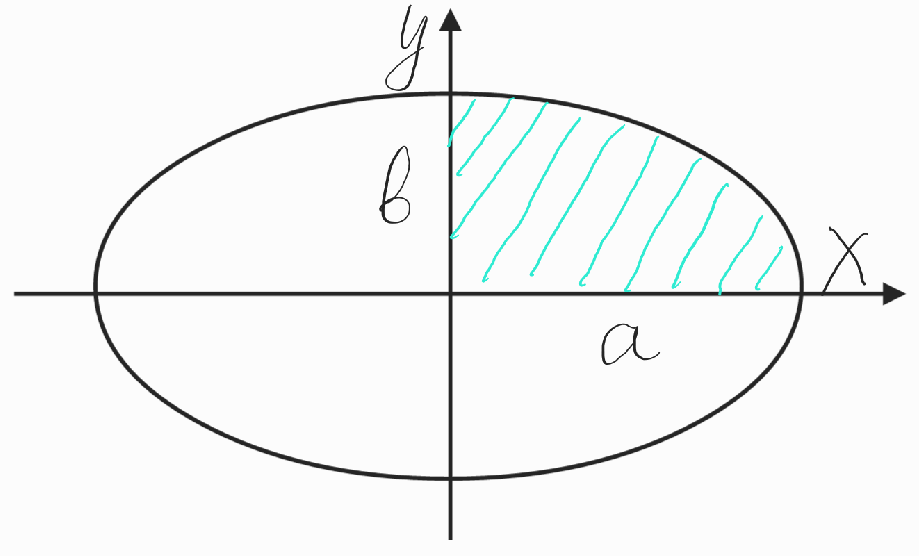
\includegraphics[width=\linewidth]{14_elips.pdf} 
        \end{minipage}
    }
    Вообще, эллипс - это кривая, но здесь речь идёт про площадь множества, ограниченного ей. Если \( a, b\) - полуоси эллипса, то найдём площадь множества 
    \[ E = \left\{ \dfrac{ x^2}{ a^2}+ \dfrac{ y^2}{ b^2} \leq 1\right\}\]
    Т.к. эллипс делится осями координат на 4 симметричные части, будем считать часть одной из них (заштрихованной), а ответ получим умножением на 4. 
    \[ S\left( E\right)=4\left( E \cap \left\{ x \geq 0, \;y \geq 0\right\}\right) = 4S(E_1)\]
    Площадь \(E_1\) будем считать как площадь подграфика функции, заданной уравнением \\
    \( \dfrac{ x^2}{ a^2}+ \dfrac{ y^2}{ b^2}=1\) в первой координатной четверти. 
    \[ y= b\;\sqrt[]{1- \dfrac{ x^2}{ a^2}}\]
    \[ S\left( E_1\right)= \displaystyle\int\limits_{ 0}^{ a} b \;\sqrt[]{1- \dfrac{ x^2}{ a^2}}dx \underset{\tilde{x}= \frac{ x}{ a}}{=} ab\displaystyle\int\limits_{ 0}^{ 1} \sqrt[]{1- \tilde{x}^2}d \tilde{x} \underset{ 
        t=\arcsin{ \tilde{x}}}{=} ab\displaystyle\int\limits_{ 0}^{ \frac{ \pi}{ 2}} \cos^2tdt= \dfrac{ \pi}{ 4}ab\]
    \[ S\left( E\right)= \pi ab\]
    Так мы заодно проверили, что площадь круга равна \( \pi r^2\).
\end{example}
\end{document}